\documentclass{article}
\usepackage[utf8]{inputenc}
\usepackage{amssymb}
\usepackage{tikz}
\usepackage{amsmath}
\usepackage{relsize}
\usepackage{mathtools}
\usepackage{textcomp}
\usepackage{eurosym}
\usepackage{graphicx}
\usepackage[autopunct=true]{csquotes}
\usepackage{chngcntr}
\usepackage{float}
\usepackage{tikz}
\usepackage{booktabs}
\usepackage{multirow}

\title{Labbook \\ Learning in Social Networks}
\author{Roman Oort 12189030\\ r.s.oort@gmail.com\\[1cm]{\normal Supervisor: Adrian Haret}}
\date{\today}
\DeclareMathOperator*{\plim}{plim}
\begin{document}

\maketitle

\newpage

\tableofcontents

\newpage

\section{Week 3}
\subsection{8/4/2021}
Started implementing network generation. Generated networks need to be aperiodic, stochastic and positive.

The code is contained in the Network class, at the moment containing the code for generating a network, adhering the to previously mentioned constraints, and the ability to grow that network. Furthermore a basic function was added to verify the generated networks do indeed converge. 

To grow the network an incremental approach was used, to ensure that the networks would satisfy the constraints at every time step. This worked by generating a square, zero, array which was a single agent larger than the previous array. The contents of the old array were then copied into this new array to maintain the same structure between iterations of the network.\newline
This method was indeed successful in creating networks that satisfy the aforementioned conditions.

However, this method was replaced in favour of a slightly different, though still incremental, updating procedure. Instead of generating an entirely new array at every time step the function was adjusted to expand the already existing network by concatenating a new row and column the already existing array. This adjustment lead to an $\sim 10 \times$ speed up in the generation time.

To ensure that the generated networks are strongly connected at every time step as each agent $i$ gets added they are guaranteed to receive both an incoming and outgoing link as they are added to the network. The receiving and sending agents for these links are chosen randomly, from an uniform distribution from the agents already present in the network.

As a side-effect this gives a natural bias towards the older agents in the network, w.r.t. degree distribution. Those agents that are present longer in a society will tend to have more connections than newcomers.

As this is just the basis for the network all weights in the network are equal.

To ensure the network is aperiodic the first agent in the network is guaranteed to get a self-link, meaning a weight to itself. For all other agents the chance whether they have a self-link is determined by an optional parameter, which defaults to 1, making it so that every agent has a self-link.

\newpage

\subsection{10/4/2021}
A function was implemented to generate the truth value of the world, and the signals sent to the agents.
The truth of the world, $mu$, is drawn from a uniform distribution over the interval $[0, 1]$. At $t=0$ each agent receives a noisy signal, $\mu + \epsilon_i$, of this true world state, where $\epsilon_i$ is a zero-mean normally distributed variable, with $\sigma^2 = \mu^2$. As each agent gets added to the network it also adds a new noisy signal to the belief vector $\textbf{p}$.

The generation method was also altered to increase the generation speed. Instead of an incremental approach the network is created at a pre-determined size, without any weight. By iterating over the agents each agents gets their respective links added, one incoming and one outgoing, from the already present agents in the network, to ensure fully connectedness at every $t$. To use the smaller networks in the computation of the convergence one can simply take a slice of the array of the desired size.

This managed to decrease the generation time from, seemingly, polynomial to linear time, greatly decreasing the network generation time, as can be seen in figure \ref{time:2} below.
\begin{center}
    \begin{figure}[!htbp]
        \centering
        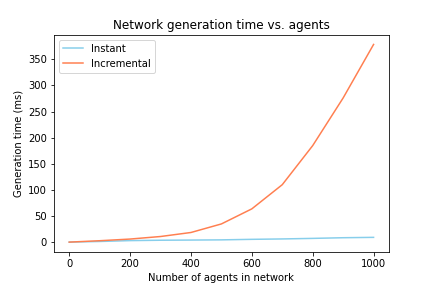
\includegraphics[width=1\textwidth]{ThesisKI/Images/GenTime2.png}
        \caption{Network Generation Time, Mean over 10 Iterations}
        \label{time:2}
    \end{figure}
\end{center}
\newpage
Additionally a method to increase the degree distribution in the network has been implemented. This uses an additional, optional, flag as parameter to use this function. When this flag is set to true, when generating the links for the network, each agent is assigned an additional, ranndom, number of incoming and outgoing links. These numbers are drawn randomly, from a 2 mean normal distribution, with $\sigma^2=1$, which are then rounded to integers. Then for the determined number of additional links the other agents involved in the link are drawn randomly, from a uniform distribution over the agents in the \emph{entire} network. This increases the degree distribution off the overall network and slightly decreases the bias on the earlier agents in the network, while not removing it entirely. The results can be seen in figure \ref{degree:increase} below.
\begin{center}
    \begin{figure}[!htbp]
        \centering
        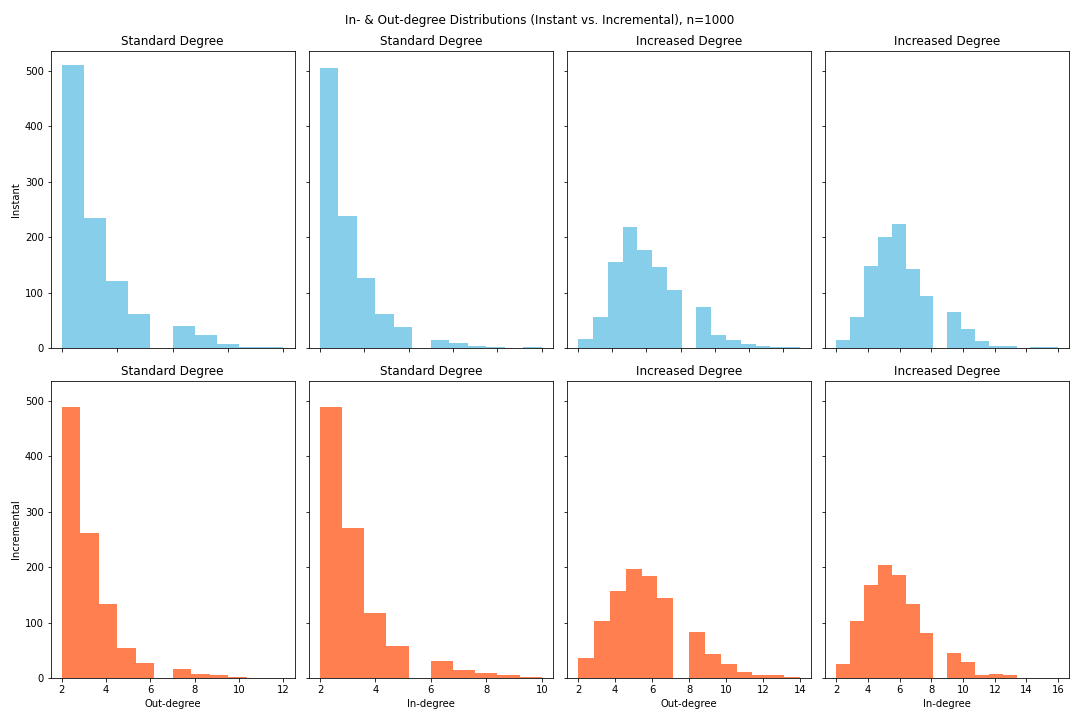
\includegraphics[width=1\textwidth]{ThesisKI/Images/IncrementalVSInstantDegree.png}
        \caption{Degree Distribution Comparison}
        \label{degree:increase}
    \end{figure}
\end{center}

\newpage
\subsection{11/4/2021}
\subsubsection{Old Functions}
The functions to generate the plots for the timing of the network generation and the degree distribution were moved to separate functions. This way one can be used without the results of the other.

Some quality of life features were added to the generation time plotting function. Optional parameters are included to determine whether the plot should be saved, to which path the plot should be saved, how many iterations should be used to average the time of the generation, and finally a parameter to determine the step size when generating the networks, which can be used to in- or decrease the resolution of the plot.\newline
Furthermore, documentation and comments were added to the function.

Comparable QoL features, like the save path, whether the plot should be saved, and whether the plot should be showed, were added to the function for generating the degree distribution plots. \newline
Furthermore the option was added to determine which generation style should be used for the network. The generation type does not have an incredibly significant impact on the degree distribution but the option was added for the sake of completion. \newline
When the parameter instant is set to true it will generate a plot with only networks that were generated using the, faster, instant generation method, see figure \ref{degree:instant}. \newline
When the incremental parameter is set to true it will generate a plot of the degree distribution of an incrementally generated network, see figure \ref{degree:incremental}. \newline
When both are set to true it will generate a plot comparing them both, see figure \ref{degree:increase}.

\subsubsection{Degree Per Agent}
Furthermore a function was added that generates a barplot of the degree of each agent. This shows how the degree of the agents as the network grows, providing insight in the, desirable, bias towards the earlier agents in the network. Using an additional parameter allows switching between instant and incremental generation. Furthermore, one can choose to use only the increased or decreased generation, or compare the two.

To ensure the generated plots were not limited to small networks while remaining readable the function takes the average degree of every $x$ agents, where $x$ is a parameter that can be set manually. This allows the examination of larger network $(n>30)$ while still retaining a readable resolution on the graph.
\newpage
\subsection{12/4/2021}
The in- and out- degree were switched to ensure they represented the correct measure, which they accidentally did not do earlier.

The instant network generation has been updated to handle the ability of growing an existing network. This is done by applying the method previously used to grow the networks incrementally over a larger amount of agents. This allows the network to be grown in steps of own choosing, i.e. by steps of 10, 100, 1000, etc. This update made the incremental growing method redundant as this functions workings can be replicated using the instant generation method with a step size of 1.

To reflect the new-found redundancy of the incremental network generation all functions were updated to no longer use this function. As no advanced functionalities were implemented as of yet this only concerns the functions used to generate the plots.

Furthermore some testing was done with different probability distributions to explore which different probability distributions can be used to generate the additional degrees of the agents.

\newpage

\subsection{13/4/2021}
The network generation function has been updated to include the ability to generate undirected network. To accomplish this the generation function was updated so that, when the links for an agent were being added, instead of choosing separate agents for the incoming and outgoing links, one agent was chosen to establish both an incoming an outgoing relation with. This was also done for the procedure for increasing the degree.

To allow further customization of the degree of agents the function was changed to allow the passing of a numpy probability distribution function, and its accompanying parameters. This was done by allowing the probability function to be passed as an optional parameter, whose default is a normal distribution with $\mu=2, \sigma^2=1$. The parameters of the chosen distribution are given in a list.

Furthermore a function was added which, using the networkx package, allows for a graph representation of a network, an example of which can be seen in figure \ref{graph:degree} below.
\begin{center}
    \begin{figure}[!htbp]
        \centering
        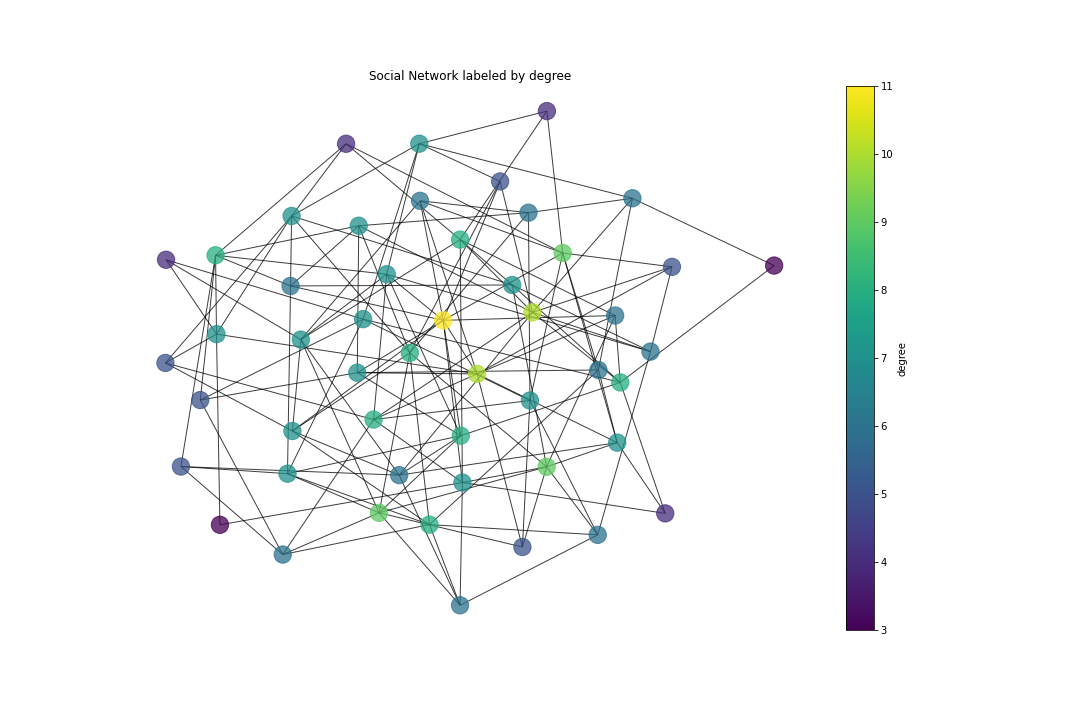
\includegraphics[width=1.3\textwidth]{ThesisKI/Images/DegreeGraph.png}
        \caption{Graph representation of network}
        \label{graph:degree}
    \end{figure}
\end{center}
As can be seen this function shows a network as a graph structure, where the nodes are the agents in the network and the edges are the links between them. This function allows for more insight in the structure of the generated networks and allow for useful visualizations. One can choose between viewing either a directed network, where the directed edges are shown using arrows, or undirected networks. Furthermore, the nodes can be labeled based on different attributes, like the degree, both in and out, the degree as a fraction of the total degree. Another option is to label the agents according to how much their opinion differs from the assumed truth in the network. This function will later be expanded to give the ability to show how many agents are able to be reached by each agents after $t$ steps, and how many steps it takes for each agent to reach every other agent. One can also choose whether or not to include the nodes or the edges in the drawing, which can be useful to reduce clutter in the visualization.

\subsection{16/4/2021}
Using the interactivity widgets of jupyter notebook the function to visually display the network was made interactive. Using this widgets several options were included in the plots, such as choosing the layout of the graph, whether or not to label the nodes or show the weights of the links. The main advantage of using this interactivity widget is the ability to generate a visualization that differs slightly without first generating an entire network, this allows the visualization of the growth of the network as more and more agents get added.

\subsection{15/4/2021}
Added implementation for 3 different ways of weight initialization: based on agent beliefs, based on the overlap in the neighbours, and randomly generated weights.

The initialization based on the beliefs looks at the difference in opinion between every two agents, the bigger this difference, the less weight the agent places on the link between them. To efficiently do this the initial belief vector was stacked, columnwise, $n$ times, where $n$ is the amount of agents in the network, and its transpose was computed. This transposed belief matrix was then subtracted from the regular belief matrix, which results in a grid containing the difference in opinion between any two agents. As the truth and the private beliefs were taken to lie on the interval $[0,1]$ the difference between these two can never exceed $1$. Then, to obtain the weights from these difference, the absolute values of these difference were then subtracted from $1$, which as these differences cannot exceed $1$ will always lie on the interval $[0, 1]$. This resulting matrix was then multiplied, elementwise, with the given adjacency matrix, containing only ones to indicate a link and zeros everywhere else, to apply the weights to the link in the network. However, as the difference between any two agents could be equal to $1$, which could result in the deletion of a link, possibly making the network no longer strongly connected, the weights were multiplied by a given factor on the interval $[0, 1]$.

The initialization using the overlap in neighbours is based on the principle that agents are aware of the structure of the network, or at least the network in close proximity to them. Under this assumption an agent would place less weight on one of its neighbours if there is a large overlap between their neighbours, as this would mean they receive a lot of the same information from the same agents. Therefore there would be little new information shared between them, making this information less valuable. This was implemented by iterating over each agent present in the network and finding their neighbours by counting the non-zero elements in their respective row. This was repeated for each of the neighbours. The overlap between these sets was then computed as a fraction of the length of the first agents set of neighbours. This fraction would then be multiplied by a given factor on the interval $[0, 1]$ to ensure total overlap between agents would not delete any links. This, discounted, fraction of overlap would then be inserted into a matrix at the coordinates of the respective link. This resulting matrix would then be subtracted from the original adjacency matrix to place less weights on those links with more overlap.

Finally the random initialization simply generates an array of the same shape as the original and fills it with values sampled independently from a given probability distribution, by default a uniform distribution on the interval $[0, 1]$.

\subsection{17/5/2021}
The function for the overlap initialization of the weights was changed to work as previously, as the earlier implemented version would occasionally result in negative weights or delete links.

Due to some memory issues when trying to create a $10,000 \times 10,000$ array a cell was added to use Google Colab integration in an attempt to work around this limit. Furthermore the ability to choose the initialization of the weights with the interactive network visualization plot was added, allowing for the swapping of weights on the fly.

Finally the ability to label the links based on their was added, and the option to view the links at a specified time $t$.

\subsection{18/4/2021}
Look into the first implementations of converging the networks. These functions were created by iteratively multiplying the original weight matrix with itself. After this multiplication the, element-wise, difference between the matrix at time $t-1$ and $t$ would be computed. All of these difference would be summed, and when this sum approaches zero, within a sufficiently small tolerance, the iteration would stop, resulting in both the converged matrix, and the time $t$ at which the matrix achieved convergence. However, these computations would take a very long time as the network size, and time $t$, increased.

\newpage

\section{Week 4}
\subsection{19/4/2021}
No significant functions were implemented, however, developments were made in the more technical aspects, w.r.t. the computations speed and memory consumption of the operations and networks.

The integration between google colab and the interactivity widget used in the notebook is spotty, so another solution had to be found for dealing with the memory issues of the local machine. After testing once again the limitation proved to be a temporary one, by my best guess caused by the long time between kernel restarts. This allowed to use my local machine to generate large networks, up to at least $30000 \times 30000$ agents, which however did take a large amount of space, not to mention computation time on these networks grew exceedingly large.

In an  attempt to speed up performance of the matrix operations cupy was installed, which allowed the use of CUDA to speed up matrix operations of both the numpy and scipy packages, to use the NVIDIA GeForce 2070 Max-Q of my local system. Furthermore, the use of the sparse matrix representation was investigated to reduce memory usage of the large, mainly empty, networks.

\begin{table}[H]
    \centering
    \begin{tabular}{lllll}
        \toprule
        Matrix Type\\ ($10000 \times 10000$) & \multicolumn{2}{c}{Normal} & \multicolumn{2}{c}{Sparse}\\
        \midrule 
        Device &\textbf{CPU} & \textbf{GPU} & \textbf{CPU} & \textbf{GPU} \\
        \midrule
        Time (s) & 113.56 & 133.43 & 2589.00 & - \\
        \bottomrule
    \end{tabular}
    \label{table:exp_time}
    \caption{Matrix exponentiation times (1000th power)}
\end{table}

As can be seen in table \ref{table:exp_time}, which shows the elapsed time in raising the adjacency matrix of a network with 10,000 agents to the 1,000th power, using the GPU does not result in a large speed up. This is most likely caused by the time associated with transferring the matrix between the CPU and GPU. Furthermore, exponentiation of the sparse matrix directly is significantly more time-consuming then raising a dense matrix to the same power.

Besides the exponentiation time the various generation times of the model were also taken into consideration, and can be seen in figures \ref{CPU:standard}, \ref{CPU:increased} and \ref{GPU:all}.
In these figures it can be seen that, when generating networks with the standard, bare minimum, degree per agent, there is hardly any difference between the different generation methods. However, when the networks are generated with the increased degree it is clear that non-sparse, CPU generation is significantly faster than both GPU generation and sparse generation.

\newpage

\subsection{21/4/2021}

The draw function has been altered to allow the size of the drawn network to go up to a thousand nodes. The previous limitation of a 100 nodes was set in place to prevent the visualization becoming too cluttered. However, to circumvent this issue the size of the plot is now determined dynamically, dependent on the size of the network shown. To grown along with the size of the plot the font-size is also determined dynamically. Below the visualization of networks of 400 and 1000 can be seen, in figure \ref{network_400:increased} and \ref{network_1000:increased} respectively.
\begin{center}
    \begin{figure}[!htbp]
        \centering
        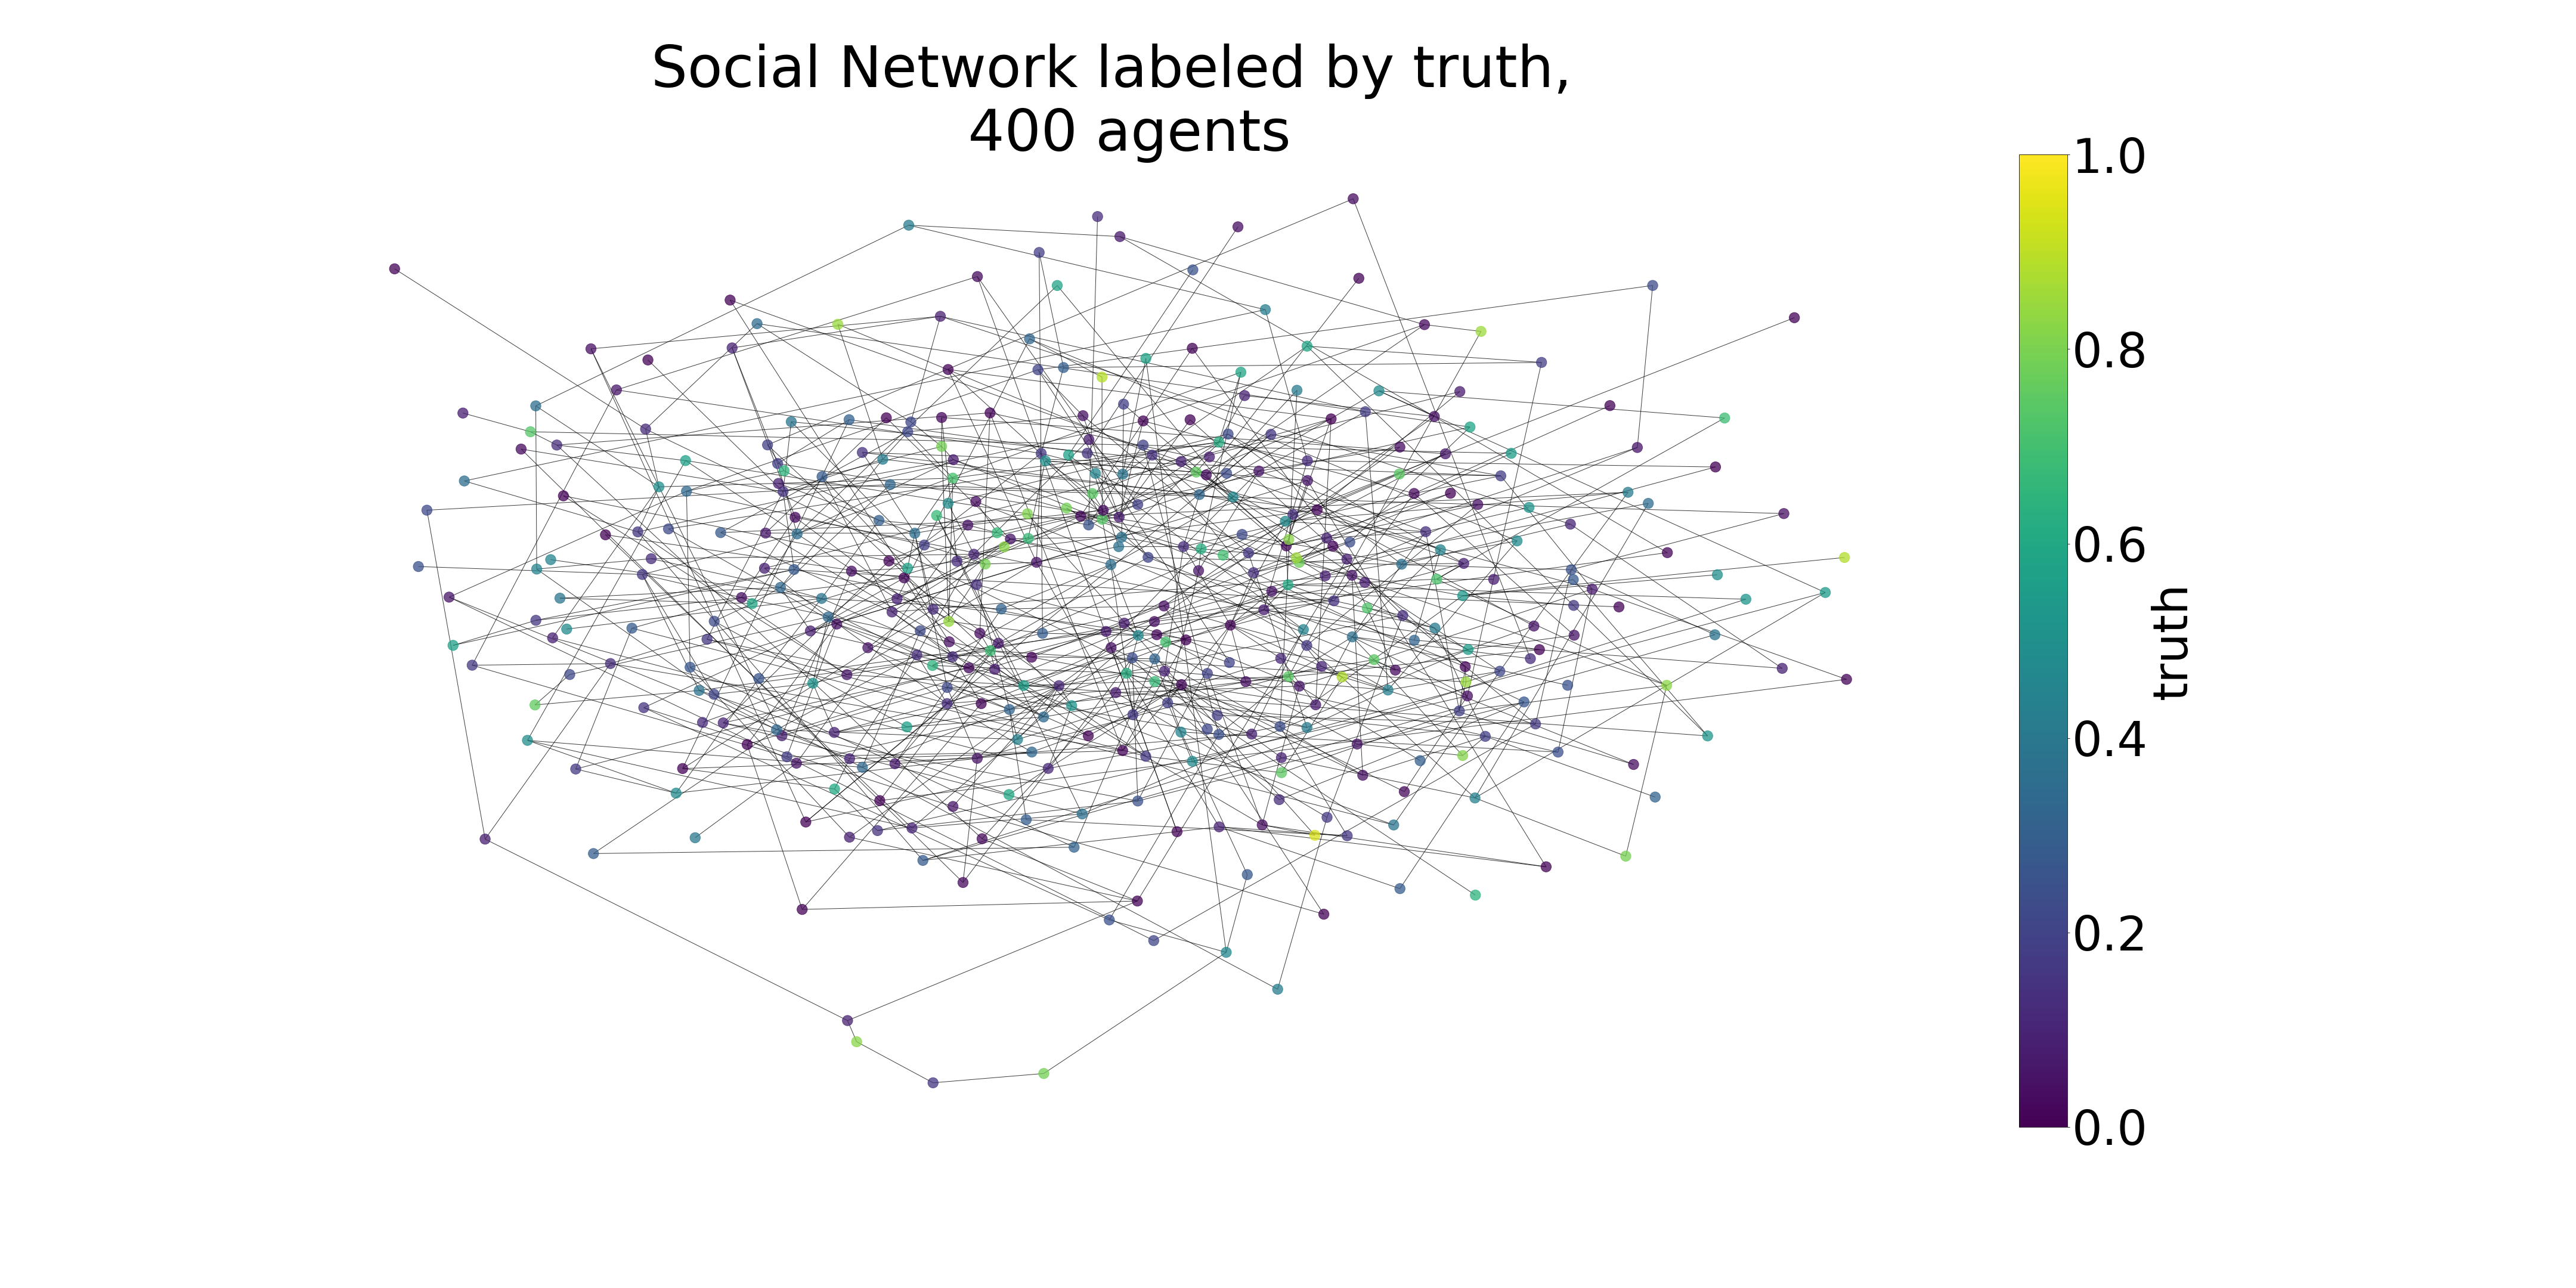
\includegraphics[width=.8\textwidth]{ThesisKI/Images/Network400UnInc.png}
        \caption{Undirected Network, Increased Degree}
        \label{network_400:increased}
    \end{figure}
\end{center}

\begin{center}
    \begin{figure}[!htbp]
        \centering
        \includegraphics[width=.8\textwidth]{ThesisKI/Images/Network1000UnInc.png}
        \caption{Undirected Network, Increased Degree}
        \label{network_1000:increased}
    \end{figure}
\end{center}

\newpage

Furthermore a function was added to visualize the progression of the convergence of the current network. First this function plotted the progression of the standard deviation and the mean of the belief vector as time progressed. However, later it was decided that plotting only the standard deviation would give a better impression of the progression of the convergence, as this measure would approach zero as the network converges. However this version of the function allowed the plotting of only a single initialization function at a time, which is rather limiting if the goal is to compare performance of convergence of these initializations. Therefore the function was altered again to be able to compare all the different weight initializations. In figure \ref{convergence:comparison} the result on a directed network, with standard degree, can be seen.

\begin{center}
    \begin{figure}[!htbp]
        \centering
        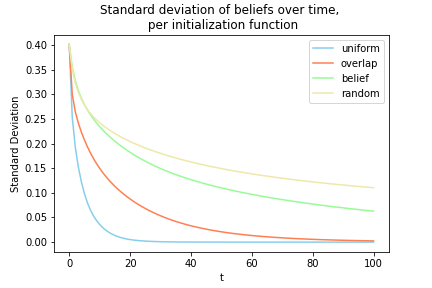
\includegraphics[width=.8\textwidth]{ThesisKI/Images/Convergence_comparison_std_dir.png}
        \caption{Directed Network, Standard Degree}
        \label{convergence:comparison}
    \end{figure}
\end{center}

This figure was chosen as it highlights the different convergence speeds between the initialization function. However, when a different type of network was chosen the curves became more similar, or differed more. Therefore the another goal is to implement a function that compares the convergence speeds of different network types. However, from a first glance analysis it appears that uniform initialization of the weights leads the network to converge the most rapidly. This makes sense as all other initialization methods serve only to reduce the weights placed on other agents, inhibiting the spread of information through the network.

\newpage

\subsection{22/4/2021}
Added a function to plot the comparison of the convergence of different network types, i.e.: directed, undirected, increased degree or standard degree. This function uses the basis of the function that compares the convergence of the different weight initializations. A helper function was added that fills a given axis object with the wanted data, which works the same as the function from yesterday, but instead of immediately plotting the graph it returns the axis object. This allows the visualizations of the different networks to be viewed in a single subplot structure, which makes it easier to compare the different workings. An example of this visualization can be seen in figure \ref{convergence:networks} below:

\begin{center}
    \begin{figure}[!htbp]
        \centering
        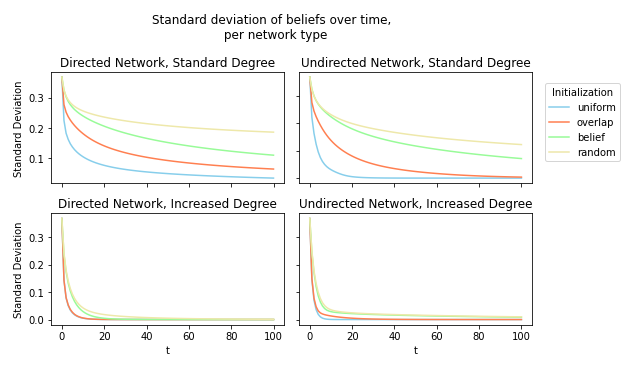
\includegraphics[width=1\textwidth]{ThesisKI/Images/ConvergenceComparison.png}
        \caption{Directed Network, Standard Degree}
        \label{convergence:networks}
    \end{figure}
\end{center}

Furthermore the function that plots the convergence of the current network was also updated to work with the function that generates the axis. This allowed to have one main function to generate the axes of these plots, reducing duplicate code.

Finally computing the convergent belief of a network was reconsidered. The method previously used was to raise the interaction matrix to a certain power, until the change in belief became negligible. However, as the networks grew larger this required more and more computation power. An earlier attempt used the eigenvector of the network, as the eigenvector corresponding to the eigenvalue $\lambda=1$ can simply be multiplied with the belief vector to obtain the convergent belief. However the earlier attempt went wrong due to a misunderstanding about the functioning of the scipy package eigh function (assuming the row eigenvectors to be the rows of the returned matrix instead of the columns). However, this computation is not entirely perfect as the returned eigenvalue is not always strictly positive, which causes some slight deviations in the computation of the belief, though this difference never exceeds $.01$.

\subsection{23/4/2021}

Another option was added to the function for drawing the network. The nodes can now also be labeled by the time it takes for them to be reached, or reach, every other agent in the network. This was done by iteratively multiplying the network with itself, and at each time step note which agents had a link to every agent in the network.

Looked into the computation of eigenvectors once more. Process can be sped up greatly by using the sparse matrix function for eigenvector calculation. This function has the ability to specify the number of eigenvectors that should be returned, and allows to specify which eigenvectors they should be. As we are interested only in the eigenvector of $\lambda=1$, which is the largest eigenvalue, we can simply compute the single eigenvector corresponding to the largest eigenvalue. This allows to computation to speed up greatly: for a $10000\times 10000$ matrix the time to compute the eigenvectors goes from $\approx$ 20 seconds to $\approx$ .03 seconds.

Furthermore the lack off convergence to wisdom was also more carefully examined and the most likely cause appears to be the generation of the beliefs. Currently all beliefs are generated as $p_i^{(0)} = \mu + e_i$, where $i$ is a zero mean error term. However, the beliefs are taken to lie on the interval $[0, 1]$, but the method of generation does not guarantee this interval. It is possible for an error term to be generated that, when summed with $\mu$, falls outside this interval. To ensure the beliefs fall in the proper interval they are normalized to this interval. This is accomplished using value normalization:
\begin{equation}
    x_{i, norm} = \frac{x_i - y_{min}}{y_{max} - y_{min}}
\end{equation}
Where $ y_{min}$ and $y_{max}$ are the lower and upper bound of the new interval respectively.
However, as a consequence of this normalization the mean of the beliefs are shifted which in turn throws of the convergence, as the networks tend to convergence to the mean belief of the network, or at close to the mean. As can be seen in figure \ref{wisdom:nonorm} below.
\newpage
\begin{center}
    \begin{figure}[!htbp]
        \centering
        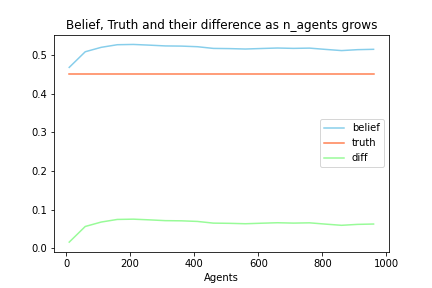
\includegraphics[width=.7\textwidth]{ThesisKI/Images/WithoutNormalizedTruth.png}
        \caption{Degree Distribution, Instant}
        \label{wisdom:nonorm}
    \end{figure}
\end{center}

However, the solution to this issue seems to be normalize the assumed truth of the network over the same interval as the beliefs. As the mean of the, non-normalized, belief vector should approach the truth of the network, as this as used as the basis for the private signals at $t=0$, normalizing the assumed truth to the same interval should shift this over to remain the mean of the beliefs. Applying this normalization does seem to solve the lack of convergence as can be seen in figure \ref{wisdom:norm} below.
\begin{center}
    \begin{figure}[!htbp]
        \centering
        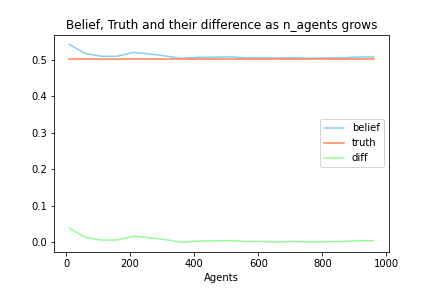
\includegraphics[width=.7\textwidth]{ThesisKI/Images/WithNormalizedTruth.png}
        \caption{Degree Distribution, Instant}
        \label{wisdom:norm}
    \end{figure}
\end{center}

\newpage

\section{Week 5}

\subsection{26/4}

Added another option to the visualization function that labels the nodes based on their time to prominence, or in other words, the lowest $t$ at which they receive information from every agent. For directed networks the nodes a distinction is made between incoming prominence and outgoing prominence. However, in undirected networks these two measures are the same.

This was done taking the current matrix that was given as input to the draw function and multiplying it with the original matrix at each step, simulating the updating rule. As soon as every entry in the matrix becomes non-zero this process stops. During this multiplication process it was stored when each row or column was entirely non-zero for the first time, which was then used as a label for the nodes in question.

\subsection{27/4}

Added another label to the visualization function, the $t$-step prominence. This shows the minimum weight, in case of directed networks either incoming or outgoing, of the connections of an agent at a given $t$. This was done by simply getting the minimum over the respective axes for the \textbf{T} matrix at the given $t$, which had to be computed in the process anyway, therefore adding little computation time.

\newpage

\section{Remaining Figures}

\subsection{10/4/2021}

\subsubsection{Degree distribution, per generation type}

\begin{center}
    \begin{figure}[!htbp]
        \centering
        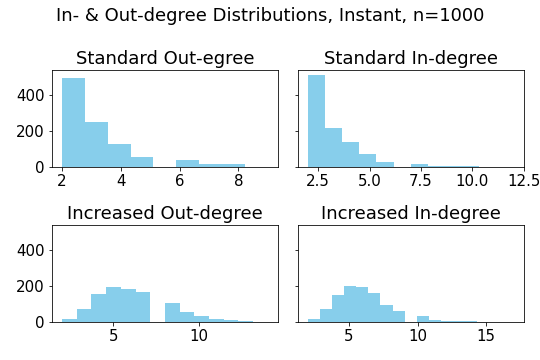
\includegraphics[width=.8\textwidth]{ThesisKI/Images/InstantDegree.png}
        \caption{Degree Distribution, Instant}
        \label{degree:instant}
    \end{figure}
\end{center}
\begin{center}
    \begin{figure}[!htbp]
        \centering
        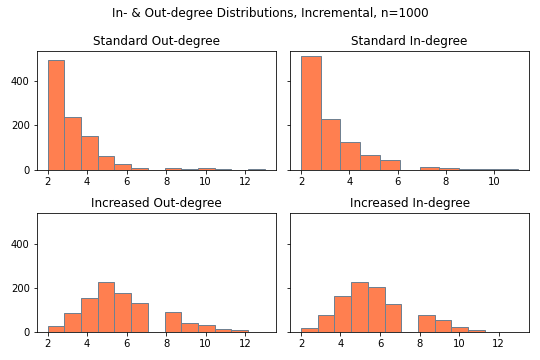
\includegraphics[width=.8\textwidth]{ThesisKI/Images/IncrementalDegree.png}
        \caption{Degree Distribution, Incremental}
        \label{degree:incremental}
    \end{figure}
\end{center}

\subsection{11/4/2021}
\subsubsection{Degree Per Agent, Instant}
\begin{center}
    \begin{figure}[!htbp]
        \centering
        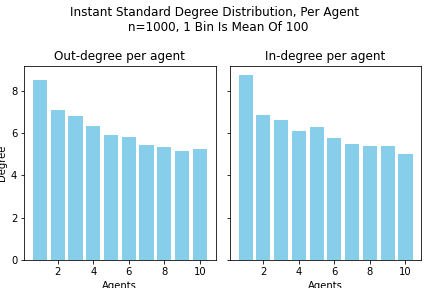
\includegraphics[width=.8\textwidth]{ThesisKI/Images/IncreasedPerAgentInstant.png}
        \caption{Average Degree Count, Instant, Increased}
        \label{DPA:InsInc}
    \end{figure}
\end{center}
\begin{center}
    \begin{figure}[!htbp]
        \centering
        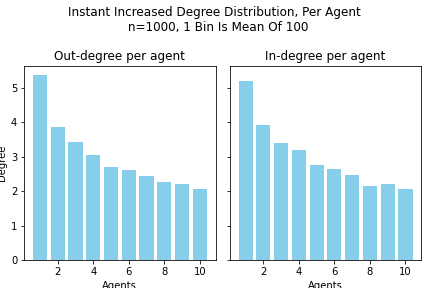
\includegraphics[width=.8\textwidth]{ThesisKI/Images/StandardPerAgentInstant.png}
        \caption{Average Degree Count, Instant, Standard}
        \label{DPA:InsStd}
    \end{figure}
\end{center}
\newpage
\subsubsection{Degree Per Agent, Incremental}
\begin{center}
    \begin{figure}[!htbp]
        \centering
        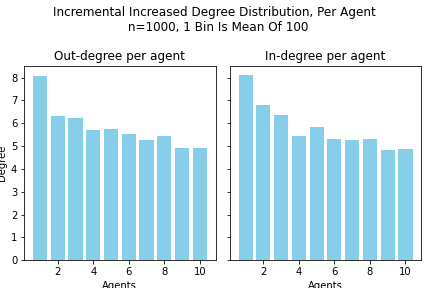
\includegraphics[width=.8\textwidth]{ThesisKI/Images/IncreasedPerAgentIncremental.png}
        \caption{Average Degree Count, Incremental, Increased}
        \label{DPA:IncInc}
    \end{figure}
\end{center}
\begin{center}
    \begin{figure}[!htbp]
        \centering
        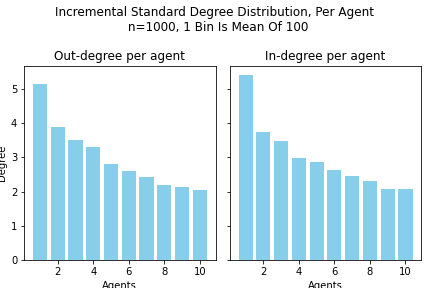
\includegraphics[width=.8\textwidth]{ThesisKI/Images/StandardPerAgentIncremental.png}
        \caption{Average Degree Count, Incremental, Standard}
        \label{DPA:IncStd}
    \end{figure}
\end{center}
\newpage
\subsubsection{Degree Per Agent, Comparison}
\begin{center}
    \begin{figure}[!htbp]
        \centering
        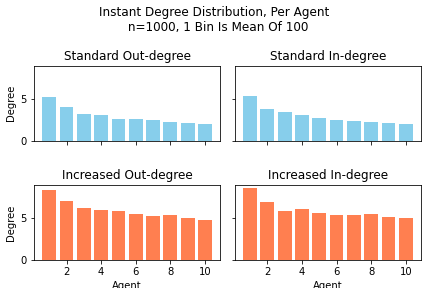
\includegraphics[width=.8\textwidth]{ThesisKI/Images/ComparisonPerAgentInstant.png}
        \caption{Average Degree Count, Instant, Comparison}
        \label{DPA:InsCom}
    \end{figure}
\end{center}
\begin{center}
    \begin{figure}[!htbp]
        \centering
        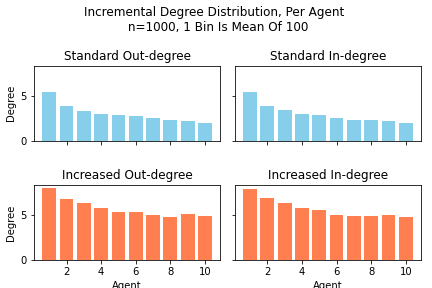
\includegraphics[width=.8\textwidth]{ThesisKI/Images/ComparisonPerAgentIncremental.png}
        \caption{Average Degree Count, Incremental, Comparison}
        \label{DPA:IncCom}
    \end{figure}
\end{center}
\newpage
\subsection{13/4/2021}
\begin{center}
    \begin{figure}[!htbp]
        \centering
        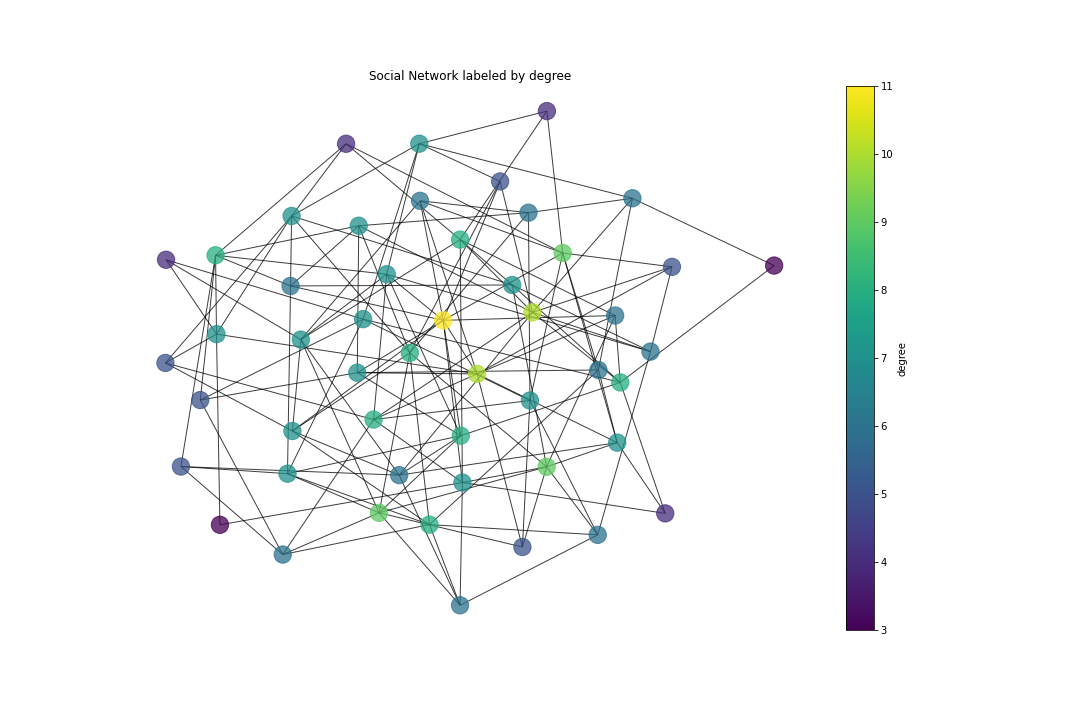
\includegraphics[width=1.3\textwidth]{ThesisKI/Images/DegreeGraph.png}
        \caption{Graph representation of network}
        \label{graph:degree}
    \end{figure}
\end{center}

\subsection{20/4/2021}
\begin{center}
    \begin{figure}[!htbp]
        \centering
        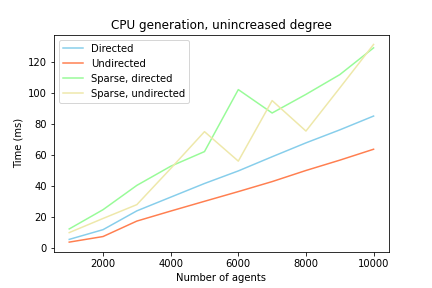
\includegraphics[width=.8\textwidth]{ThesisKI/Images/CPU.png}
        \caption{CPU generation time, standard degree}
        \label{CPU:standard}
    \end{figure}
\end{center}

\begin{center}
    \begin{figure}[!htbp]
        \centering
        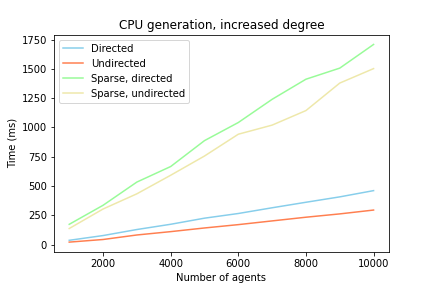
\includegraphics[width=.8\textwidth]{ThesisKI/Images/CPU_inc.png}
        \caption{CPU generation time, increased degree}
        \label{CPU:increased}
    \end{figure}
\end{center}

\begin{center}
    \begin{figure}[!htbp]
        \centering
        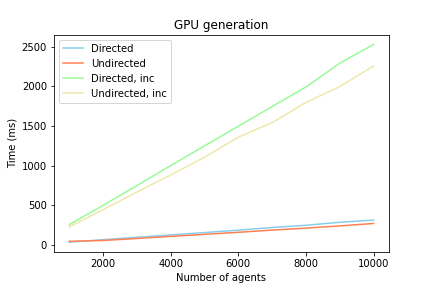
\includegraphics[width=.8\textwidth]{ThesisKI/Images/GPU.png}
        \caption{GPU generation time}
        \label{GPU:all}
    \end{figure}
\end{center}

\end{document}
